\documentclass[10pt]{article}
\usepackage[utf8]{inputenc}
\usepackage{amsmath,amsfonts,amssymb}
\usepackage{graphicx}
\usepackage{geometry}
\geometry{a4paper, margin=1in}

 \newcommand{\blds}[1]{\mbox{\scriptsize \boldmath $#1$}}
% Save the original \frac command
\let\oldfrac\frac
% Redefine \frac to behave like \dfrac
\renewcommand{\frac}{\dfrac}


\title{Radar and Remote Sensing Equation Sheet}
\date{}

\begin{document}

\maketitle

\centerline{Rachel Middleton} 

\centerline{Rachel.Middleton@colorado.edu}


\section*{Radar Fundamentals}


\begin{enumerate}

\item Transmit Signal, $T_x$ for a monostatic radar block diagram: \\
  
  
	\centerline{{$T_x (t) = A_0U(t)\cos[2\pi f(t)t +\phi_{TX}(t)]$}}
 
	where:

	$A_0$ = amplitude

	$U(t)$ = pulse train signal

	$f(t)$ = transmit frequency

	$\phi _{TX}(t)$ = transmit phase
  
  
\item Received Signal, $R_x$ for a monostatic radar block diagram: \\
  
  
	\centerline{$R_x (t) =k(A_0 U(t-\nabla t)\cos[2\pi f(t-\nabla t) + \psi] +n(t))$}
	
	where:

	$\psi$ = the sum of the phase shifts of the target and with the radar

	$k$ = is order of $10^{-18}$
  
  % Add more equations here
  
\item The Radar Power Equation

	\centerline{$P_r = \frac{P_t G_t G_r {\lambda}^2 \sigma}{(4\pi)^3 R^4}$}
	
	where:
	
	Pt – Transmitted power (at antenna terminals) [W]

	Gt – Transmitter antenna gain [unitless]

	R – Range to target [m]
	
	RCS – Target’s radar cross section (also expressed as $\sigma$) [$m^2$]
	
	Gr – Receiver antenna gain  [unitless]
	
	Pr – Received power (at antenna terminals) [W]
	
	$\lambda = \frac{c}{f}$ = wavelength [m]

\break
	The following quantities can be derived from the RPE, see ASEN5245\_01c\_Radar\_Fundamentals\_2024\_0118 for more equations

	\begin{enumerate}	
		\item Power density for an Isotropic Antenna

		\centerline{$Q_i = \frac{P_t}{4\pi R^2}$ [Watts/$m^2$]} 

		where:
	
		$Q_i$ is the incident power density for and isotropic antenna($G_t = 1$)
	
		$4 \pi R^2$ is the area of a sphere
	

		\item Radar Cross Section (RCS)

		\centerline{$\sigma (\theta,\phi) = \frac{P_{reflected}[W]}{Q_i [W/m^2]}[m^2]$}
	
		\item Radiation Scattered by a Target

		\item Power Backscattered by a Target

		\item Power Density at Receive Antenna

		\item Power Backscattered by Target

		\item Power Collected by Receive Antenna

		\item Received Power at Antenna Ports

	\end{enumerate}

\item Calculations in dB

	\centerline{$P_{dB} = 10\log (\frac{P_{linear}}{P_0})$}
	
	where:
	
	$P_{linear}$ is a value in "linear" units and $P_0$ represents the reference value (typically 1)
	
	When the reference has physical meaning, then ‘dB’ is replaced with
a special units:

Reference to milliWatts ($P_0 = 10^{-3}  W$) dBm

Reference to Watts dBW

Reference to square meters (RCS, $\lambda$, ) dBsm

Reference to isotropic radiator dBi

Reference to dipole radiator dBd

\item Pulse Radar Range

	\centerline{$R_{target} = \frac{c T_{delay}}{2}$ [m]} 
	
	where c is the speed of light, $3x10^8$
	
	
\item Pulse Radar Waveform

	$\tau$ [s] - the pulse width or duration the Tx is transmitting
	
	$T_{IPP}$ or IPP - the inter-pulse period [s], time between pulses
	
	$PRF = 1/T_{IPP}$ [Hz]  - the pulse repetition frequency
	
	Duty Cycle = $100(\frac{\tau}{T_{IPP}})$ [\%]
	
	
\item Range Resolution
	
	\centerline{$\nabla R = R_2 - R_1 = c\frac{T_2 - T_1}{2} = c\frac{\delta t}{2}$}
	
	where $\delta t$ is the minimum time such that two targets at R1 and at R 2
	will appear completely resolved

	therefore:

	\centerline{$\nabla R = \frac{c\tau}{2}$}
	
\item Unambiguous Range (Pulse Radar)

	\centerline{$R_{max} = \frac{c T_{IPP}}{2}$}
	
	Range aliasing implies that a target observed at range, $R_{obs} < R_{max}$
could have come from a different inter-pulse period
	
\end{enumerate}

\section*{Noise and Losses}

\begin{enumerate}

	\item Noise Power of a Radar System
	
	\centerline{$P_n = kT_{sys}B$ [W]}
	
	where:
	
	$P_n$ is the noise power in Watts
	
	k - Boltzmann’s constant: $1.38x10^{-23}$ [J/K], note: [J] = [Watt second]
	
	$T_{sys}$ -  system noise temperature [K]
	
	B - receiver bandwidth [Hz] (typically B ~ 1/$\tau$, where $\tau$ is the pulse width [s]

	\item Random Antenna Noise
	
	\centerline{$T_{sys} = T_{antenna} + T_e = (T_a +T_A) + T_e$}
	
	$T_a$ - External noise. Noise picked up by the antenna (e.g., Galactic
noise, sun, moon, ground and other thermal emitters. This noise is
part of the antenna temperature
	
	$T_A$ - Thermal Emission. Noise due to physical antenna temperature.
Also part of the antenna temperature
	
	$T_e$ - Receiver noise. Internally generated noise by Rx components (e.g.,
amplifiers, mixers). This noise is quantified by the Rx effective
noise temperature


	\item Radar Losses
	
	\centerline{$L_{total} = L_{sys}L_{prop}$ where $L_{total}\ge1$}
	
	Two kinds of losses may occur:
	Propagation Path Losses – losses associated with the propagation
	medium between target and radar, such as, atmospheric attenuation and
	multipath interference

	System Losses – losses within the radar system itself, such as insertion
	loss, as waves propagate through the radar system. (Losses within the
	antenna are accounted for in the antenna efficiency)
	
	effciency, $\rho$ is expressed as $L = \frac{1}{\rho}$
	
	Losses are factored into the RPE as follows:
	
	\centerline{$P_r = \frac{P_t G_t G_r {\lambda}^2 \sigma}{(4\pi)^3 L_{FSPL}^2R^4}$}
	
	where $L_{FSPL}$ is the one-way propagation loss (notice this quantity squared is the two-way propagation loss)


	\item Specific Attenuation Model for Rain
	
	see reference doc: ITU-R P.838-1
	
	\centerline{$\gamma_R = kR^{\alpha}$ [dB/km]}
	
	where $\gamma_R $is the specific attenuation for rain [dB/km]
	
	$k$ and $\alpha$ are frequency dependent constants tabulated for
horizontal (H) and vertical (V) propagation polarizations
	
	R is rain rate [mm/hr]
	
	Then, we factor these losses into the RPE as:
	
	\centerline{$P_r = \frac{P_t G_t G_r {\lambda}^2 \sigma}{(4\pi)^3 L_{FSPL}^2 L_{rain}^2R^4}$}
	
	where $L_{rain}$ is the one-way propagation loss for rain (distance * attenuation rate) (notice this quantity squared is the two-way propagation loss)
	
	Similar attenuation rates can be calculated for other atmospheric mediums, such as cloud and fog (Recommendation ITU-R P.840-3)
	
	\item Coax Cable, Insertion loss (Attenuation)
		(a system loss)
		
	
	\item Signal to Noise Ratio (SNR)
	
	\centerline{$SNR = \frac{P_r}{P_n} = \frac{P_t G^2 \lambda^2 \sigma}{(4\pi)^3 L_{sys} L_{prop}^2 R^4 kT_{sys}B}$}
	
	\item Coherent integration
	
	\centerline{$(SNR)_{coherent}(n_p) = n_p SNR(1)$}
	
	where $n_p$ is the number of consecutive pulses
	
	
	\item Maximum Detectable Range
	
	\centerline{Detection Threshold = $SNR_{min} = \frac{P_t \tau G^2 \lambda^2 \sigma}{(4\pi)^3 L_{sys} L_{prop}^2 R^4 kT_{sys}}$}
	
	\centerline{Max Detectable range  = $R_max = [\frac{P_t \tau G^2 \lambda^2 \sigma}{(4\pi)^3 L_{sys} L_{prop}^2 SNR_{min}kT_{sys}}]^{1/4}$}
	
	\centerline{min RCS = $\sigma_{min} = \frac{(4\pi)^3 L_{sys} L_{prop}^2 SNR_{min}kT_{sys}R^4}{P_t \tau G^2 \lambda^2 }$} 
	
	\item Fourier Transform (FT)
	
	The Fourier transform can be viewed as a projection onto an orthogonal basis
	function.

	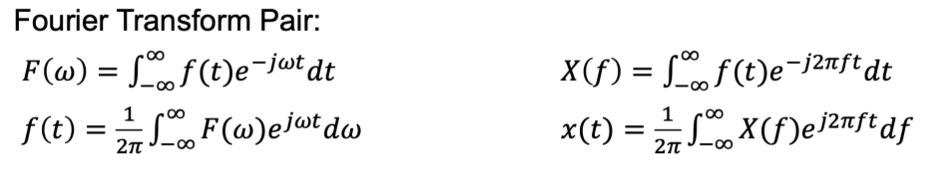
\includegraphics[width=0.99\textwidth]{figs/FT_pair.png}


	The basis functions are the complex exponentials.

	Note that both $F(\omega)$ and $f(t)$ are continuous functions and can be either 	real or complex (as with $I$ and $Q$ voltages).

	From Eulier’s Identity, we can represent cosines and sines with complex
	exponentials.

	Negative frequencies represent clockwise (CW) rotation on complex plane

	Positive frequencies represent counter-clockwise (CCW) rotation on
	complex plane 11


	Refer to ASEN5245\_Intro\_Matched\_Filter\_Compression\_013024.pdf for 		examples and further explanation.



	\item Pulse Compression Ratio [TODO]
	
	\item Decoding Phase Modulation [TODO]


\end{enumerate}

\section*{EM Basics}

\begin{enumerate}

	\item Electrostatics
	
	\begin{itemize}
	
		\item Ohms Law: $V = RI$
	
		where:
		
		V = Voltage [V]
		
		R = Resistance [$\Omega$]
		
		I = Current [Ampere]
		
		\item Electric Field
		
		$\tilde{E} = \rho \tilde{J}$
		
		where: 
		
		$\tilde{E}$ = electric field [V/m]
		
		$\tilde{J}$ = current density [A/$m^2$]
		
		$\rho$ = resistivity of the medium [$\Omega$/m]
		
		$\sigma = 1/\rho$ = conductivity 
		
		
		
		\item Coulomb's Law: $\tilde{E} =  \frac{q}{4\pi \epsilon_0 r^2}\vec{R} [V/m^2]$

		where:

		$\epsilon_0$ = Permittivity of Free Space  = $\frac{1}{36\pi}*1-^{-9}$ [Farads/m]

		Dielectric Constant = $\epsilon = \epsilon_r \epsilon_0$
		
		$\tilde{E}$ = electric field [V/m]
		
		$\tilde{D}$ = Electric Flux Desnsity: $\tilde{D} = \epsilon \tilde{E}$
		
		

		$r$ = Distance between the centers of the two charges [m]
		
		\end{itemize}
		
	\item Magnetostatics
		\begin{itemize}

		\item Biot-Savart Law: $\vec{B} = \mu \tilde{H}$

		where:

		$\tilde{B}$ = Magnetic flux density [Tesla] = $\tilde{B} = \frac{\mu_0 I}{2\pi r}$
		
		$\tilde{H}$ = Magnetic field intensity [A/m]

		$\mu_0$ = Permeability of free space \(\approx 4\pi \times 10^{-7} \, \text{T m/A}\)
		$\mu = \mu_r \mu_0$ and $\mu_r = 1$ for this class
		$I$ = Electric current [A] = $\frac{dq}{dt}$

		$\vec{r}$ = Position vector from the length element to the point of observation [m]
		\end{itemize}
		
	
		
	\item Electromagnetics
		
		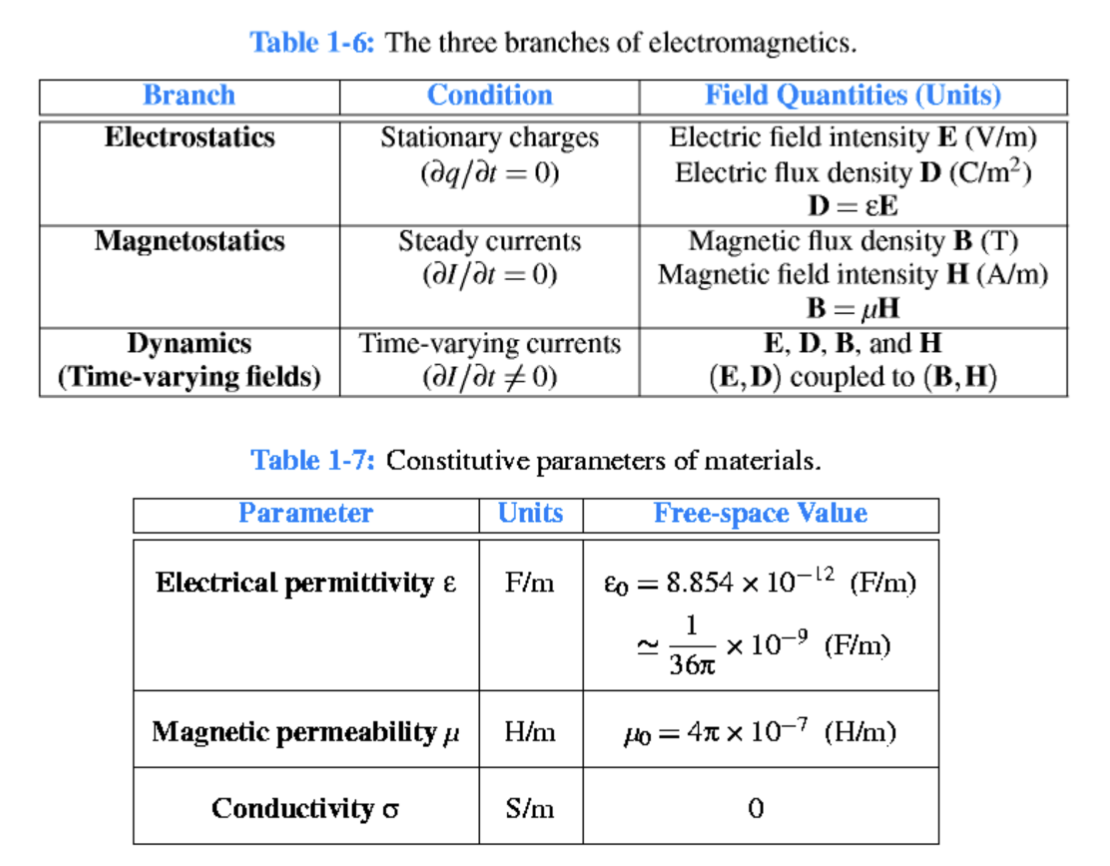
\includegraphics[width=0.99\textwidth]{figs/Electromagnetics.png}
	
	\item Maxwell’s Equations
	
	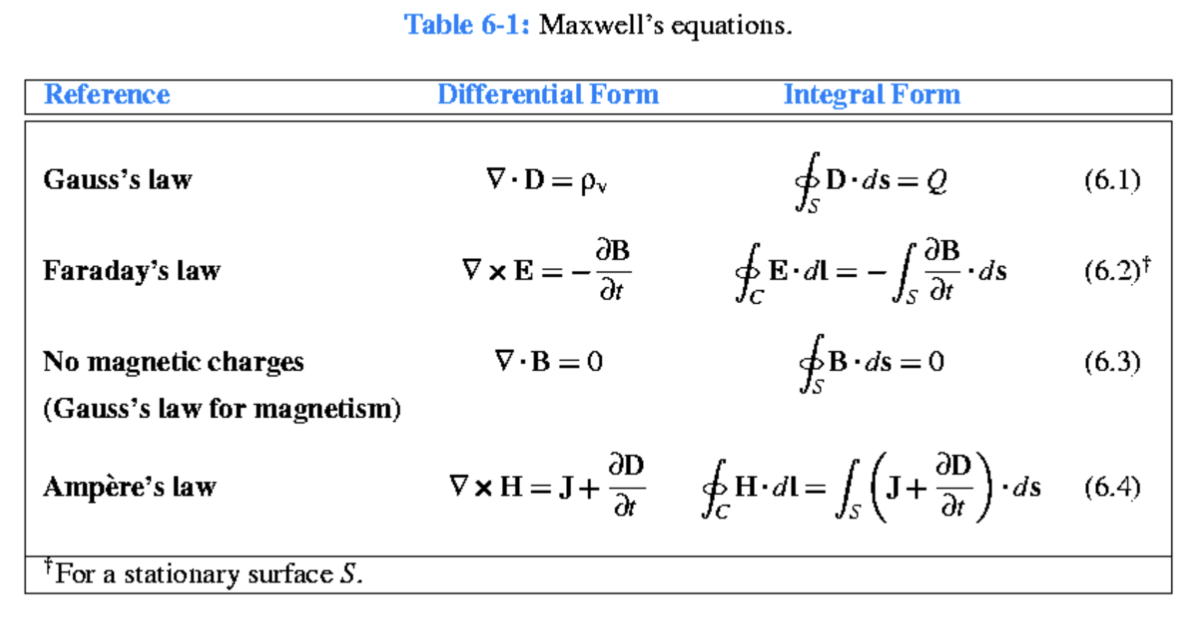
\includegraphics[width=0.99\textwidth]{figs/MaxwellsEquations.png}
	
	
	\item Phasor notation
	
	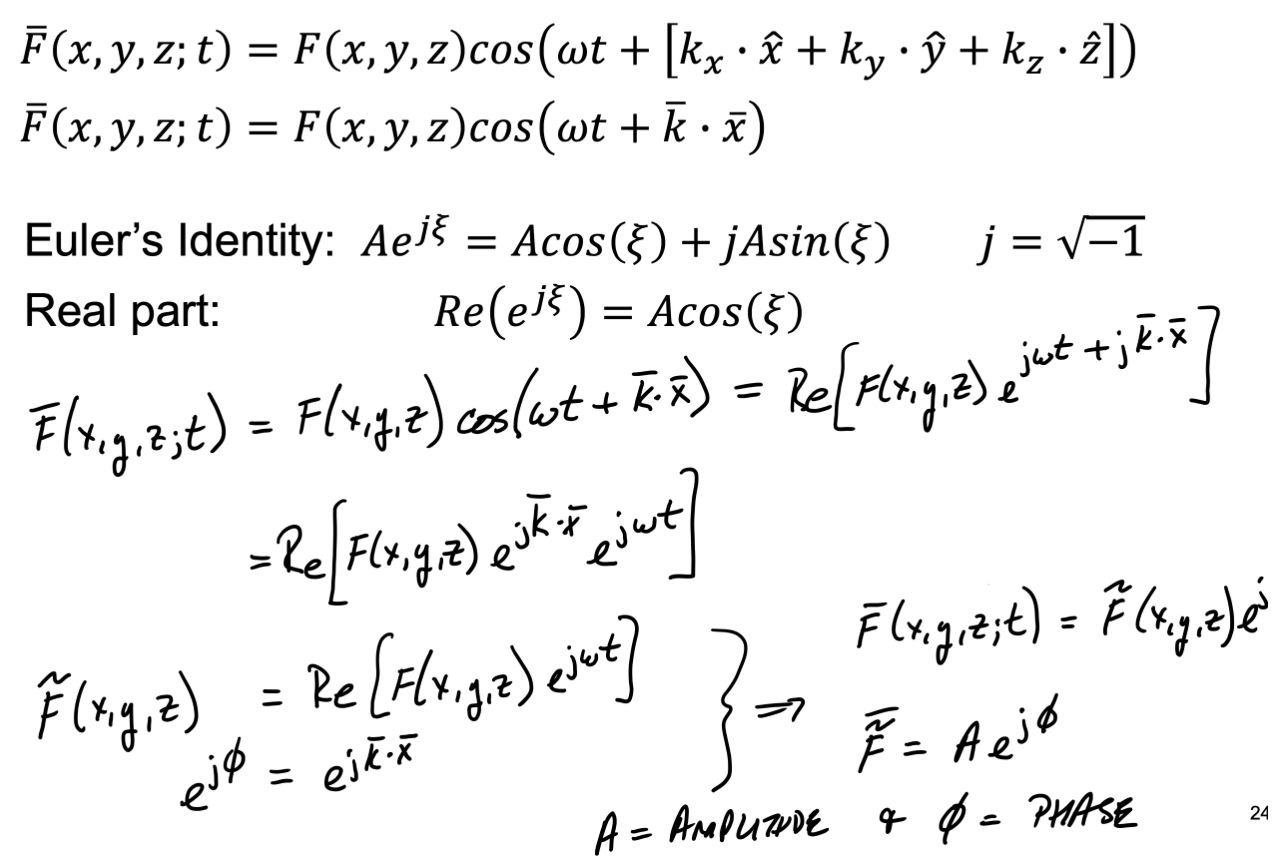
\includegraphics[width=0.99\textwidth]{figs/PhasorNotation.png}
	
	
	\item Complex permittivity
	
	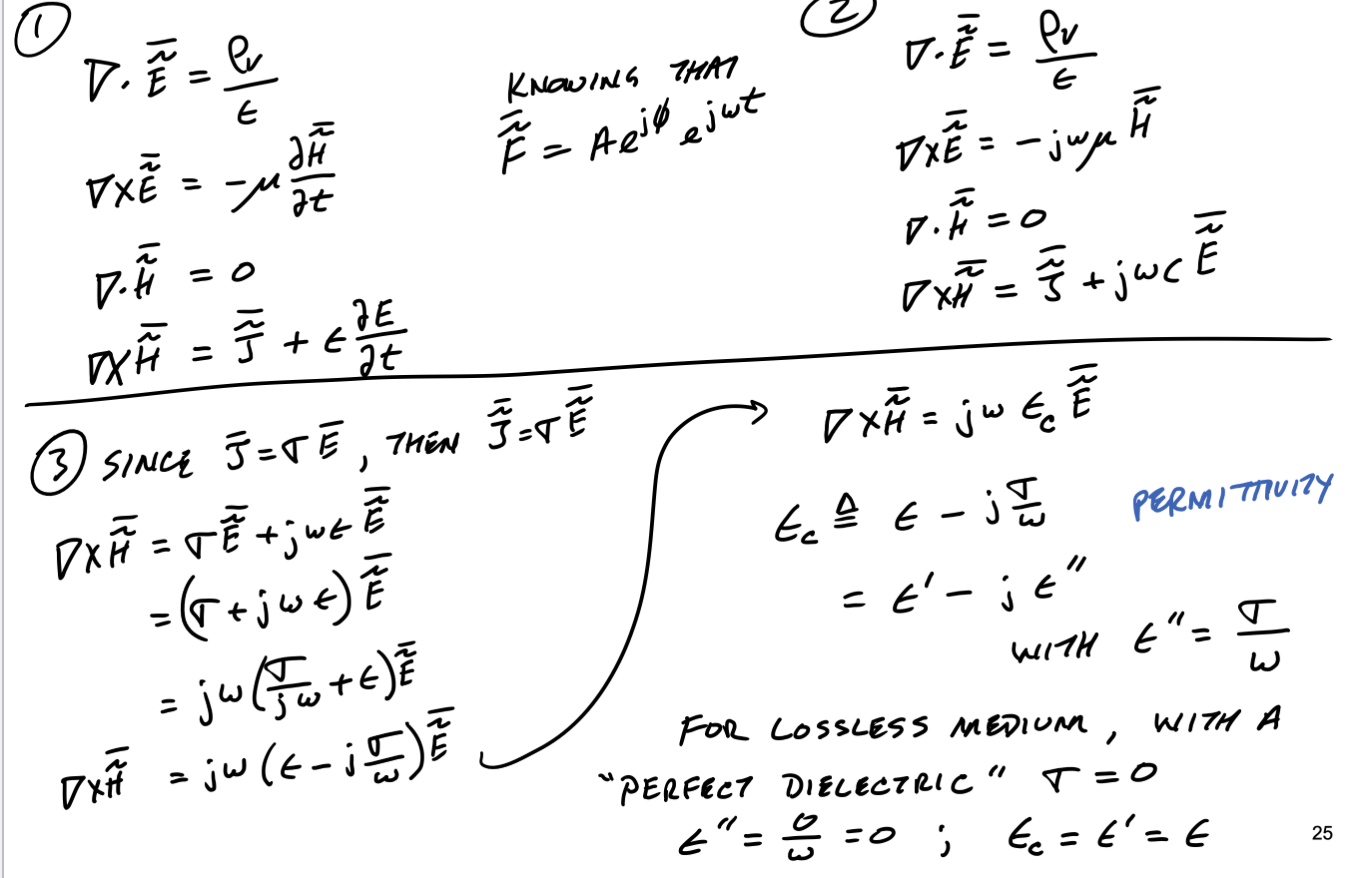
\includegraphics[width=0.99\textwidth]{figs/ComplexPermittivity.png}
	
	\item Propagating Waves
	
	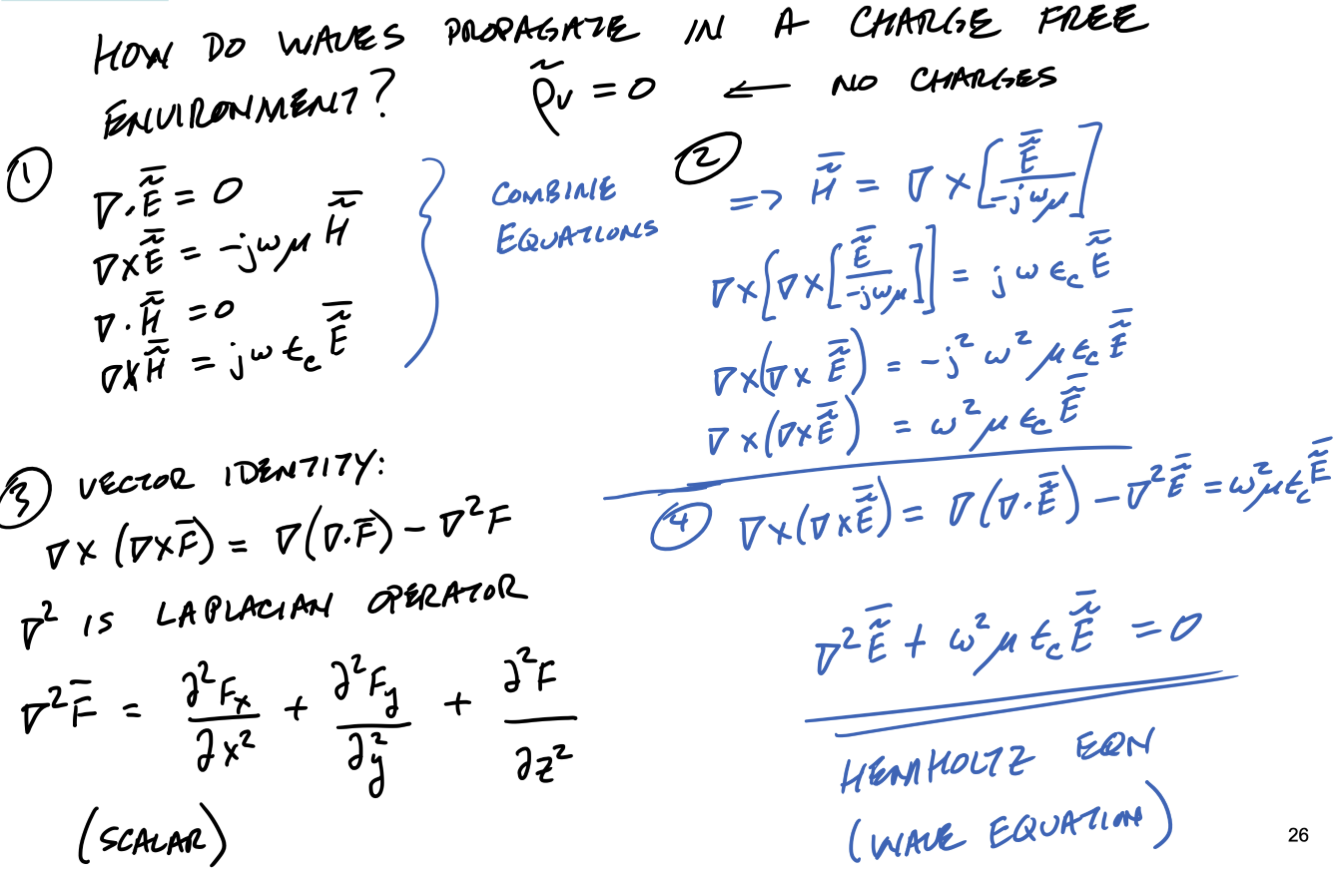
\includegraphics[width=0.99\textwidth]{figs/PropagatingWaves.png}


\end{enumerate}
\break


\section*{Wave Propagation and Scattering}

\begin{enumerate}

	\item The Homogenous Wave Equation
	
	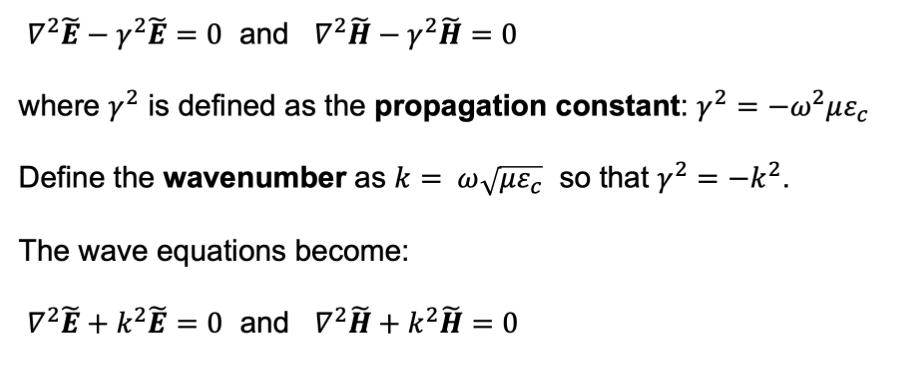
\includegraphics[width=0.79\textwidth]{figs/HomogenousWaveEqn.png}
	
	Recall from Maxwell's equations that E and H are orthogonal:
	
	\centerline{$\bar{H} = \frac{1}{\eta}\vec{k}\times \bar{E}$}
	
	\centerline{$\bar{E} = -\eta \vec{k} \times \bar{H}$}
	
	\centerline{$\eta = \sqrt{\frac{\mu}{\epsilon}}$}
	
	and $\vec{k}$ is the unit vector in the direction of propagation.
	
	\begin{itemize}
		\item One solution to the wave equation with $\tilde{E}_y = 0$ has the form:
		
		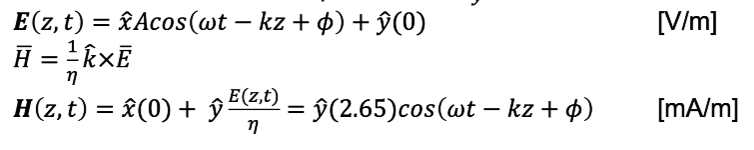
\includegraphics[width=0.69\textwidth]{figs/WaveSolution.png}
		
		
	\end{itemize}
	
	\item Propagation through multiple elements
	
	Losses of medium are usually expressed one-way path loses in dB.
	
	\centerline{$L_i = \alpha_i d_i$}
	
	where $\alpha_i$ is the attenuation coefficient [dB/km] and $d_i$ is the path length [km]
	
	Loss along the full path length is the Free Space Propagation Loss (FSPL) and is the sum of the Losses ($L_1 + L_2 + L_3 + ... = L_{total}$)
	
	\item Plane Wave Propagation in Lossless Media
	
	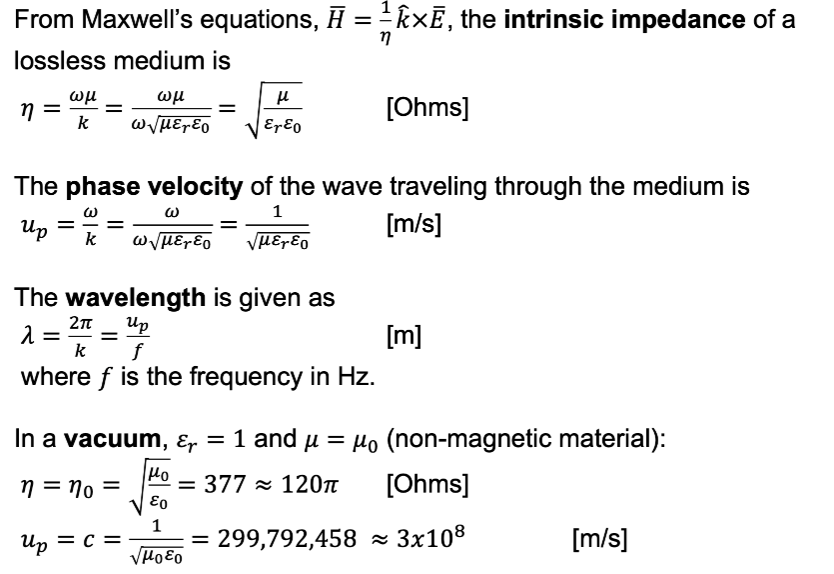
\includegraphics[width=0.89\textwidth]{figs/LosslessMedia1.png}
	
	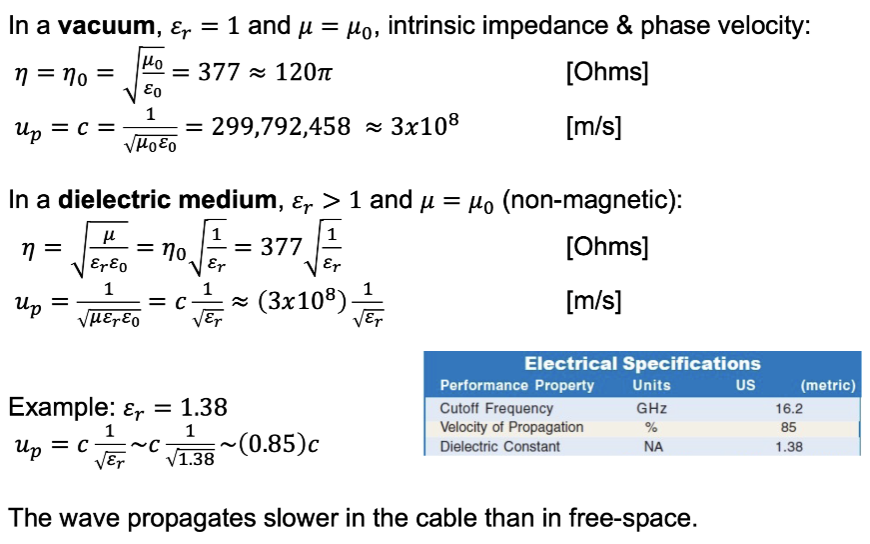
\includegraphics[width=0.89\textwidth]{figs/LosslessMedia2.png}
	
	\item Atmospheric Refraction
	
	Refraction - radio waves travel in a different direction because of the {\bf index of refraction}
	
	\centerline{The index of refraction, $n = \frac{c}{v_p}$}
	
	where c is the speed of light and $v_p$ is the phase speed of the wave in the medium \\
	
	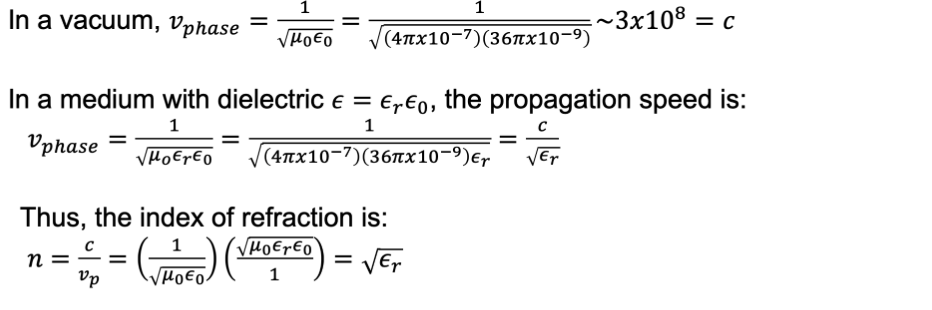
\includegraphics[width=0.79\textwidth]{figs/Refraction.png}
	
	The index of refraction is a complex quantity with real and imaginary parts ($n = \sqrt{\epsilon_r} = n' - jn''$)
	
	and is also defined as:
	
	\centerline{$n = 1 + 10^{-6}N$}
	
	where N is the refractivity
	
	\item*{Scattering}
	\begin{itemize}
	\item Refraction - waves change direction as they pass from one medium to another
	\item Diffraction - waves change direction as they pass through an opening or navigate around a barrierrr
	\item Reflection - waves bounce off barrier

	– Surface, multi-path, and plate reflection

	\item Radar cross-section
		
		For example, a plate has the cross section: 
		
		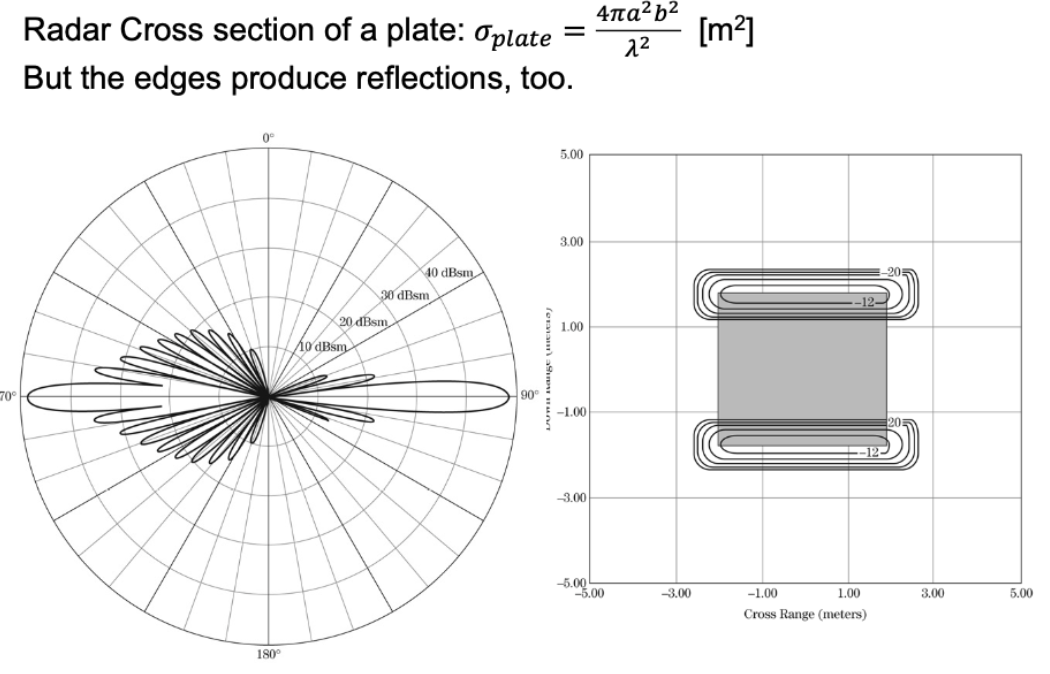
\includegraphics[width=0.69\textwidth]{figs/RCS_plate.png}
	
	\end{itemize}


\end{enumerate}


\subsection*{Antenna Properties}

\begin{enumerate}

	\item Radiation Properties
		
		\begin{itemize}
		
			\item Reciprocity
			\item Antenna Pattern
			\item Gain
			\item Polarization
			
		\end{itemize}
	\item Impedance Properties
		\begin{itemize}
			\item Radiation resistance
			\item Loss resistance
			\item Voltage Standing Wave Ratio (VSWR)
		
		\end{itemize}
		
	\item Antenna Radiated Power
	
	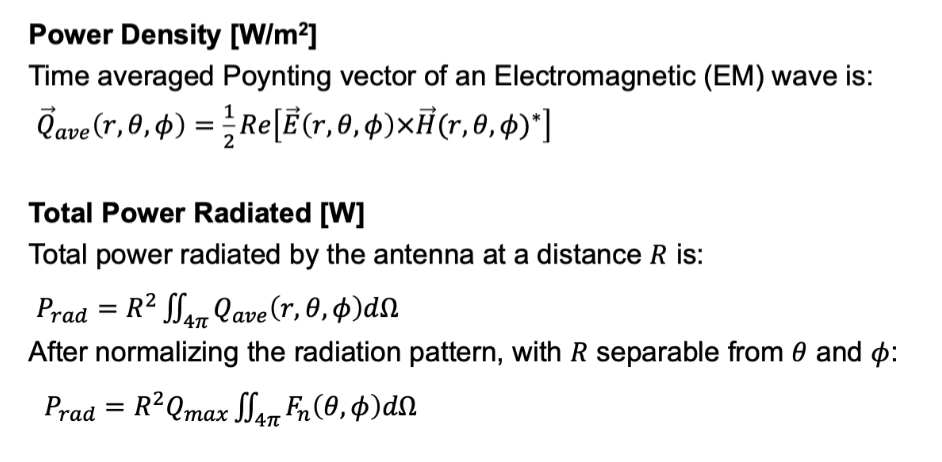
\includegraphics[width=0.79\textwidth]{figs/antennaradiatedpower.png}
	
		
		
	\item Radiation Pattern
	
		 The normalized radiation pattern is as follows:
		 
		 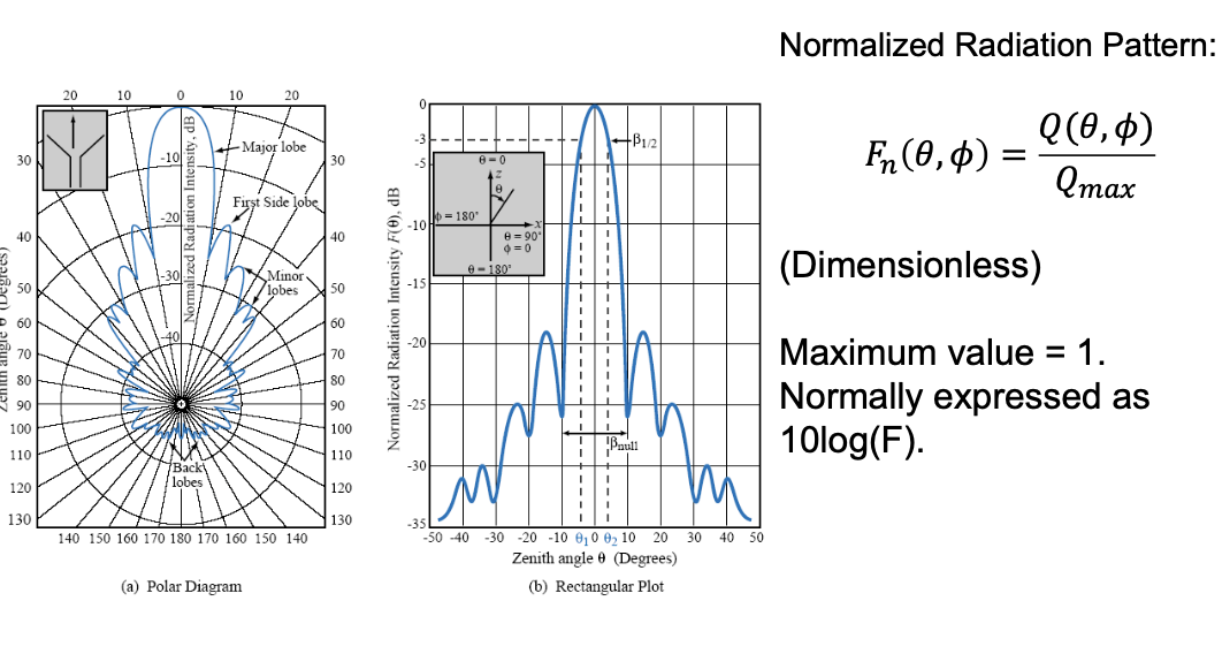
\includegraphics[width=0.79\textwidth]{figs/normalizedradiationpattern.png}
		 
		 
	\item Beam width
	
		HPBW (half power beam width) is the angle between the two angles where the poer is half of the max value. In dB, the power drops about 3 dB from the max value. In Linear Voltage, the power drops by a factor of 0.707.
	
	\item Directivity (Isotropic radiator and Pattern solid angle)
		
		How well an antenna directs energy relative to an isotropic antenna
		
		Radiation intensity, the power radiated per unit solid angle:
		
		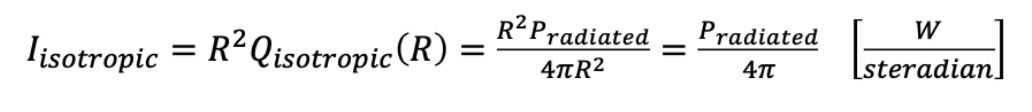
\includegraphics[width=0.59\textwidth]{figs/radiationintensity.png}
		
		And the power density at range R:
		
		$Q_{density} (R) = \frac{P_{radiated}}{\Omega_p R^2} [\frac{W}{m^2}]$
		
		where $\Omega_p$ is the pattern solid angle and can be approximated as:
		
		$\Omega_p = \theta_{HPBW} \phi_{HPBW}$
		
		{\bf Directivity, D:}
		
		$D = \frac{I_{antenna}}{I_{isotropic}} = \frac{\frac{P_{radiated}}{\Omega_p}}{\frac{P_{radiated}}{4\pi}} = \frac{4\pi}{\Omega_p}$ 
		
		Note that we make the following assumptions:
		
		\begin{itemize}
			\item Ignore all sidelobes
			\item All energy is within HPBW
			\item Power density is uniform across beam solid angle
		\end{itemize}
		
	\item Gain 
	
	Antenna efficiency, $\rho$: 
		
		$\rho = \frac{P_{radiated}}{P_t}$ 

		where $P_t$ is the power supplied by the transmitter to the antenna terminals.
		
	Gain, $G$:
	
		$G = \rho D$
		

	\item VSWR 
	
	Considered the antenna as an impedance, or the ratio of voltage to current at the feed port.
	We want to maximize the power transfer, but a VSWR of 2:1 is generally good enough:
	
	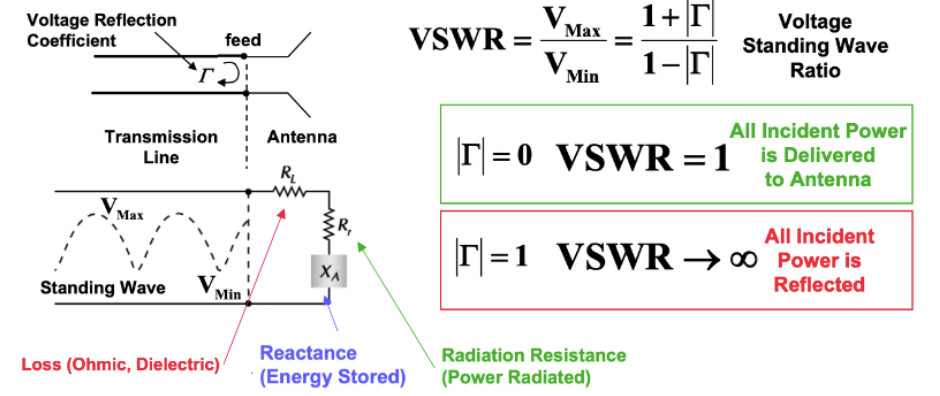
\includegraphics[width=0.79\textwidth]{figs/VSWR.png}
	
	where $\Gamma$ is the reflection coefficient
	
	
	\item Effective Aperture, $A_e$
	
	The solid angle $\Omega_p$ is related to the area an antenna would use to capture propagating power density, Q.
	
	The effective aperture is scaled by wavelength. 
	
	$\Omega_p = \frac{\lambda^2}{A_e}$
	
	Thus: $A_e = \frac{\lambda^2}{\Omega_p} = \frac{\lambda^2}{\theta_{HPBW}\phi_{HPBW}}$
	
	So Directivity, D, can also be calculated as:
	
	$D = \frac{4\pi}{\Omega_p} = \frac{4\pi}{\lambda^2}A_e$
	
	
	\item Beam Width
	
	Let beam width be a function of antenna coordinates (x,y) instead of $\theta$ and $\phi$.
	
	From $\Omega_p =  \theta_{HPBW}\phi_{HPBW} = \frac{\lambda^2}{A_e}$, we can write:
	
	$\beta_x \beta_y \approx \frac{\lambda}{l_x} \frac{\lambda}{l_y}$
	
	So, beam width is approximately: $\beta \approx \frac{\lambda}{length of antenna}$ [radians]
	
	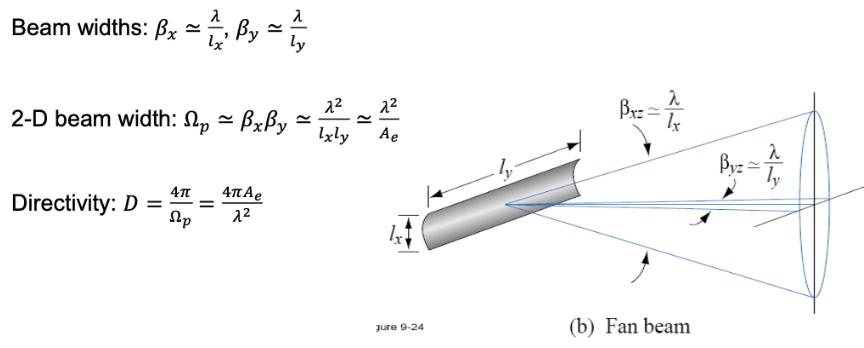
\includegraphics[width=0.79\textwidth]{figs/beamwidth.png}
	
	
	\item Physical Aperture, $A_p$
	
	For dish and horn antennas, it can be useful to relate effective and physical apertures through the aperture efficiency $\eta _{aperature}$
	
	$A_e = \eta_{aperature} A_p$

	\item Aperture illumination
	
	More amplitude taper increases the antenna beam width by factor $k_x$. and reduces the side-lobe amplitude
	
	$\beta_x = k_x \frac{\lambda}{l_x}$ 
	
	Antenna efficiency is also related to these constants:
	
	$\eta_{aperature} = \frac{1}{k_x k_y}$
	
	
	\item Polarization
	
	Types of polarizations:
	\begin{itemize}
	\item Linear polarizations (horizontal and vertical)
	
	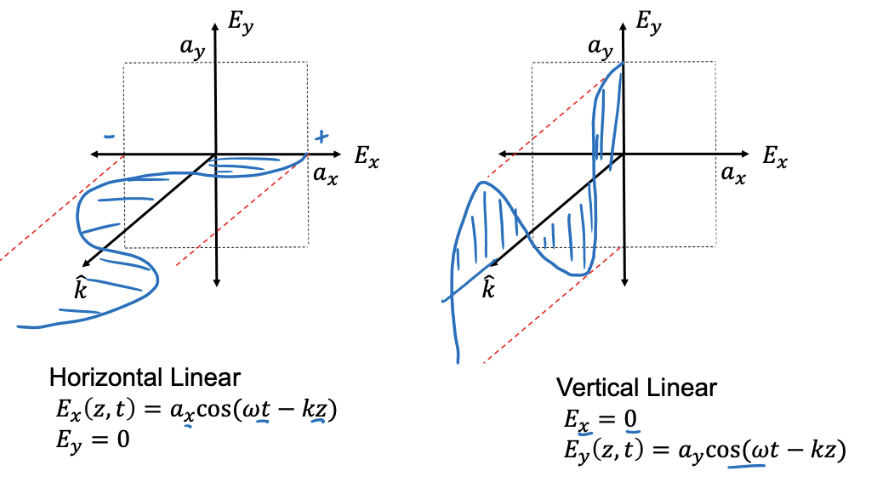
\includegraphics[width=0.69\textwidth]{figs/linearpolarization.png}
	
	\item Slant polarization
	
	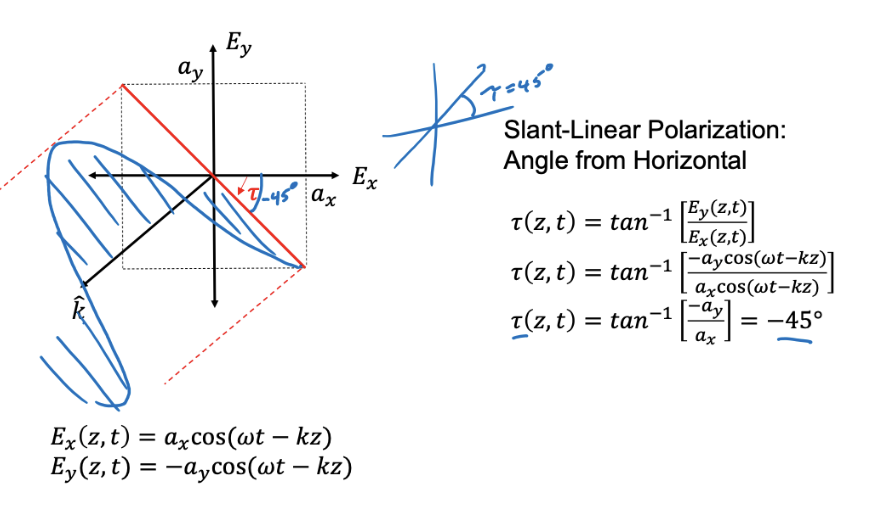
\includegraphics[width=0.69\textwidth]{figs/slantpolarization.png}
	
	\item Circular polarization
	
	Right hand circular (counter clock-wise rotation)
	
	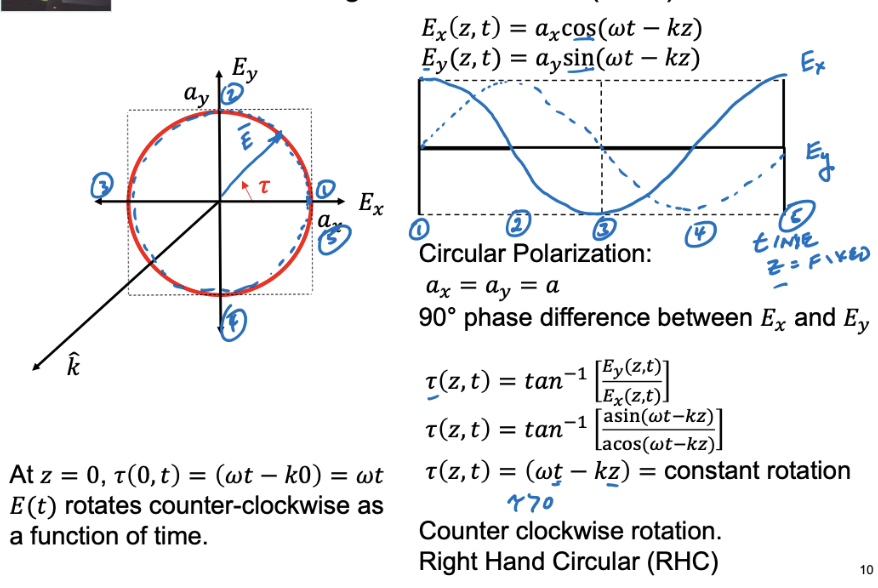
\includegraphics[width=0.69\textwidth]{figs/RHCpolarization.png}
	
	Left hand circular (clock-wise rotation)
	
	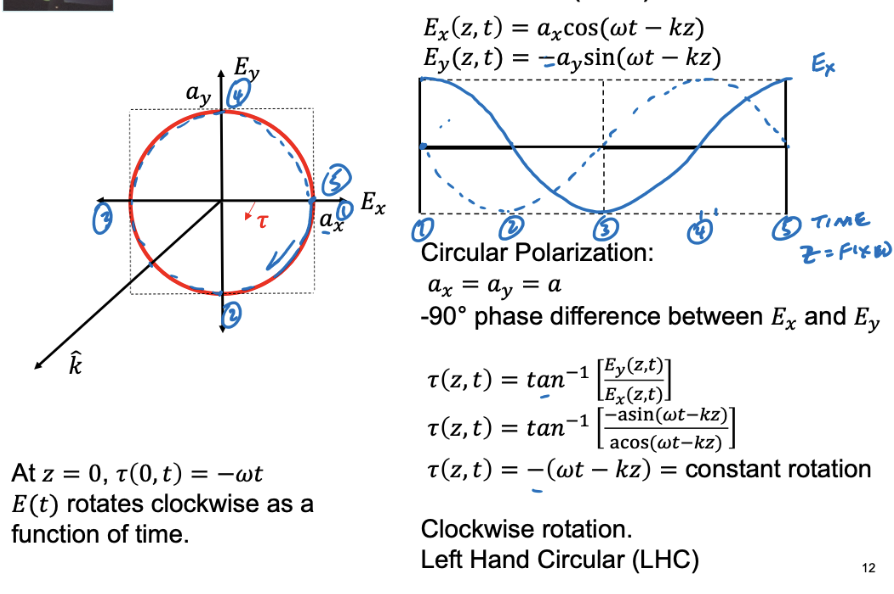
\includegraphics[width=0.69\textwidth]{figs/LHCpolarization.png}
	
	
	\item Elliptical polarization
	
	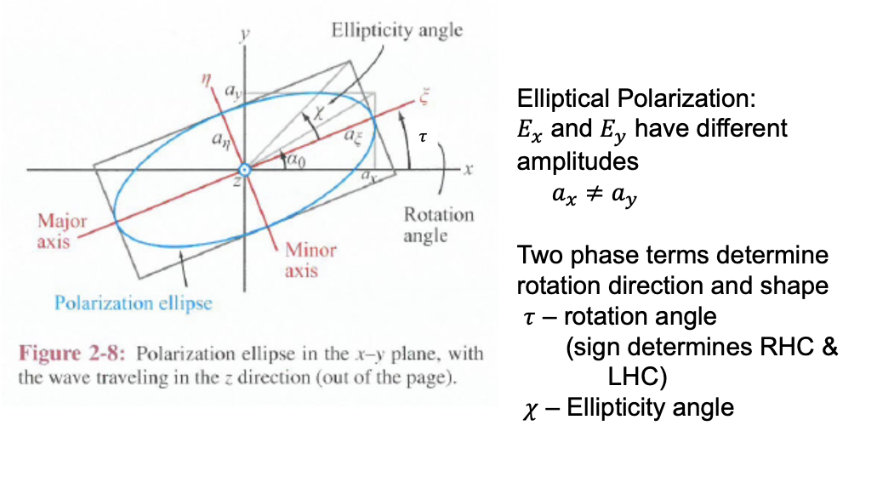
\includegraphics[width=0.69\textwidth]{figs/elipticalpolarization.png}
	
	\end{itemize}
	
	Transform between linear and circular polarizations:
	
	\includegraphics[width=0.69\textwidth]{figs/transform\_polarizations.png}
	
	
	Target Scattering Matrix
	
	A scattered wave's polarization is determined by its scattering matrix:
	
	$E^{scat} = S_{target}E^{inc}$
	
	where the scattering angle and incident angle both change the scattering matrix. In the monostatic case, the scattering angle is 180
degrees from the incident angle is called backscattering.
	
	\includegraphics[width=0.69\textwidth]{figs/scattering\_matrix.png}


\end{enumerate}


{\bf Volume Scattering}

\begin{enumerate}





\item Radar Pulse Volume

The volume of the radar resolution volume is defined by range, and the
azimuth and elevation angles of the antenna pattern.




\item Radar Cross Section of volume of distributed targets

The RCS of volume targets is the summation of RCS of the individual targets:

$\sigma_{volume} = \sigma^0 \Delta V = \sum \sigma_{targets}(i) \Delta V = \eta \Delta V$

where $\sigma^0$ is the RCS of the volume of targets per unit volume


\item Radar Power Equation for volume target scattering

The radar resolution volume (aka resolution cell) is the volume
illuminated by the radar.

\includegraphics[width=0.69\textwidth]{figs/radar\_resolution\_volume.png}

The power returned at the antenna terminals by a volume target is given as:

\includegraphics[width=0.69\textwidth]{figs/radar\_eqn\_volume\_targets.png}

The SNR for a volume target is given as:

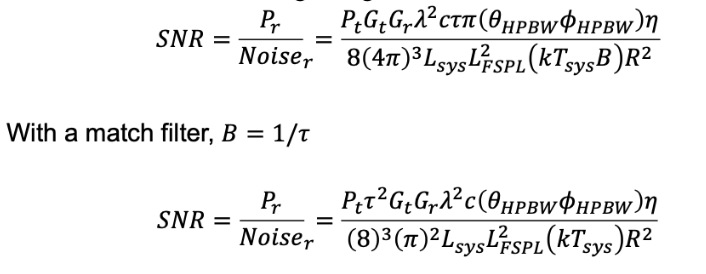
\includegraphics[width=0.69\textwidth]{figs/SNRVolume.png}

where $\tau$ is the pulse length.




\item For more on estimating RCS depending on the radar grazing angle, see 

ASEN5245\_Scattering\_01\_Volume\_Surface\_Particle\_022724.pdf



\item Scattering Regions


\end{enumerate}






























\end{document}
